\chapter{Results}\label{chapter:results}

This chapter discusses the experimental results. First, some notable insights and results from the synthetic Zipf-like workload generation are explored in \Cref{res:zipf-gen}. Then, we dive into the most relevant findings of this work, regarding the cache simulations performed in \Cref{res:cache-sim}.

\section{Synthetic Data Generation}\label{res:zipf-gen}

This section examines some insights gained from generating the synthetic Zipf-like workloads used to simulate web traffic for the cache simulations.

\subsection{Theoretical Zipfian Distributions}\label{theoretical-zipf}

As previously discussed in \Cref{bkg: zipfian-distributions}, Zipfian distributions are characterized by the skewness parameter $\alpha$, which dictates the frequency with which a few popular items are accessed compared to a vast number of less popular items. Lower values of $\alpha$ result in a more uniform distribution where all items have nearly equal probability of being accessed. When $\alpha=1$, the probability of accessing an item is exactly inversely proportional to its rank. For $\alpha>1$, the distribution becomes more heavily skewed; the most popular items are accessed dramatically more often, and the long tail of unpopular items becomes even flatter and less likely to be requested. 

\begin{figure}[h!]
    \centering
    \caption{Rank-Frequency Plots for Zipfian Distributions (linear and log scales)}
    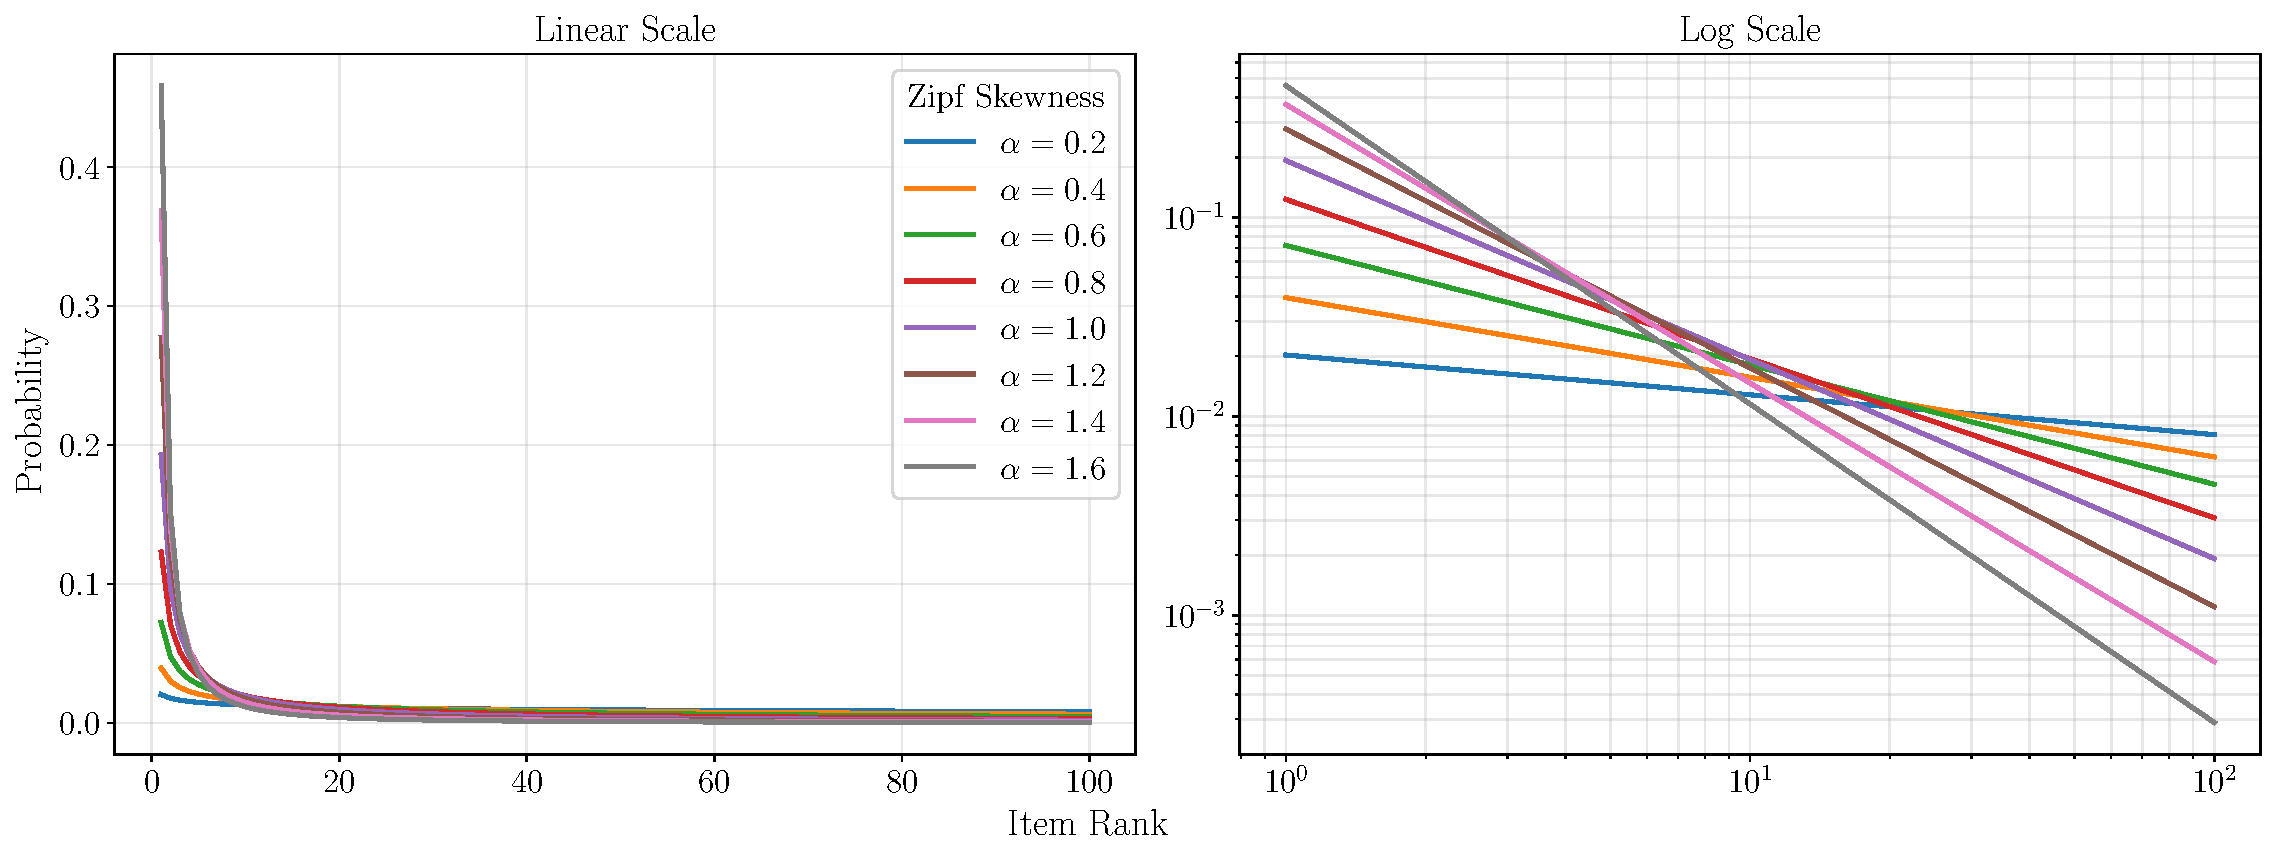
\includegraphics[width=\linewidth]{figures/workloads/zipfian_curves_all_both_no_title.pdf}
    \label{fig:zipf-alpha}
\end{figure}

The effect of the skewness parameter $\alpha$ is best visualized by the rank-frequency plots in \Cref{fig:zipf-alpha}. The linear plot demonstrates the shape of Zipfian distributions; items with a lower rank have a higher probability of being sampled. We observe from the log plot that the relationship between rank and probability is a straight line, confirming the inverse power-law relation inherent in a Zipfian distribution. The slope of each line is directly related to the $\alpha$ value; a larger negative slope corresponds to a larger $\alpha$, and a shallower negative slope corresponds to smaller values. This visually demonstrates how $\alpha$ controls the decay rate of the distribution, with a higher value indicating that the probability drops off more quickly with increasing rank.


\subsection{Actual Zipf-like Workloads Generated}

The generated Zipf-like workloads were sampled from Zipfian distributions with differences in (1) skewness parameter $\alpha$ and (2) working set size, which is the set of unique requested items. Due to the probabilistic nature of sampling, the size of the actual working set of the generated workloads differs from the target working set indicated at sampling time. In fact, the difference between the two shows to have been heavily impacted by the choice in $\alpha$, as can be seen from the boxplot in \Cref{fig:boxplot-actual-theoretical-ratio}.

\begin{figure}[h!]
    \centering
    \captionsetup{justification=centering}
    \caption{Boxplot of Actual/Theoretical Working Set Ratio By Zipfian Skewness Parameter $\alpha$. The {\color{PineGreen}\textbf{green}} line represents the median and the {\color{blue}\textbf{blue}} box represents the interquartile range (middle 50\% of data).}
    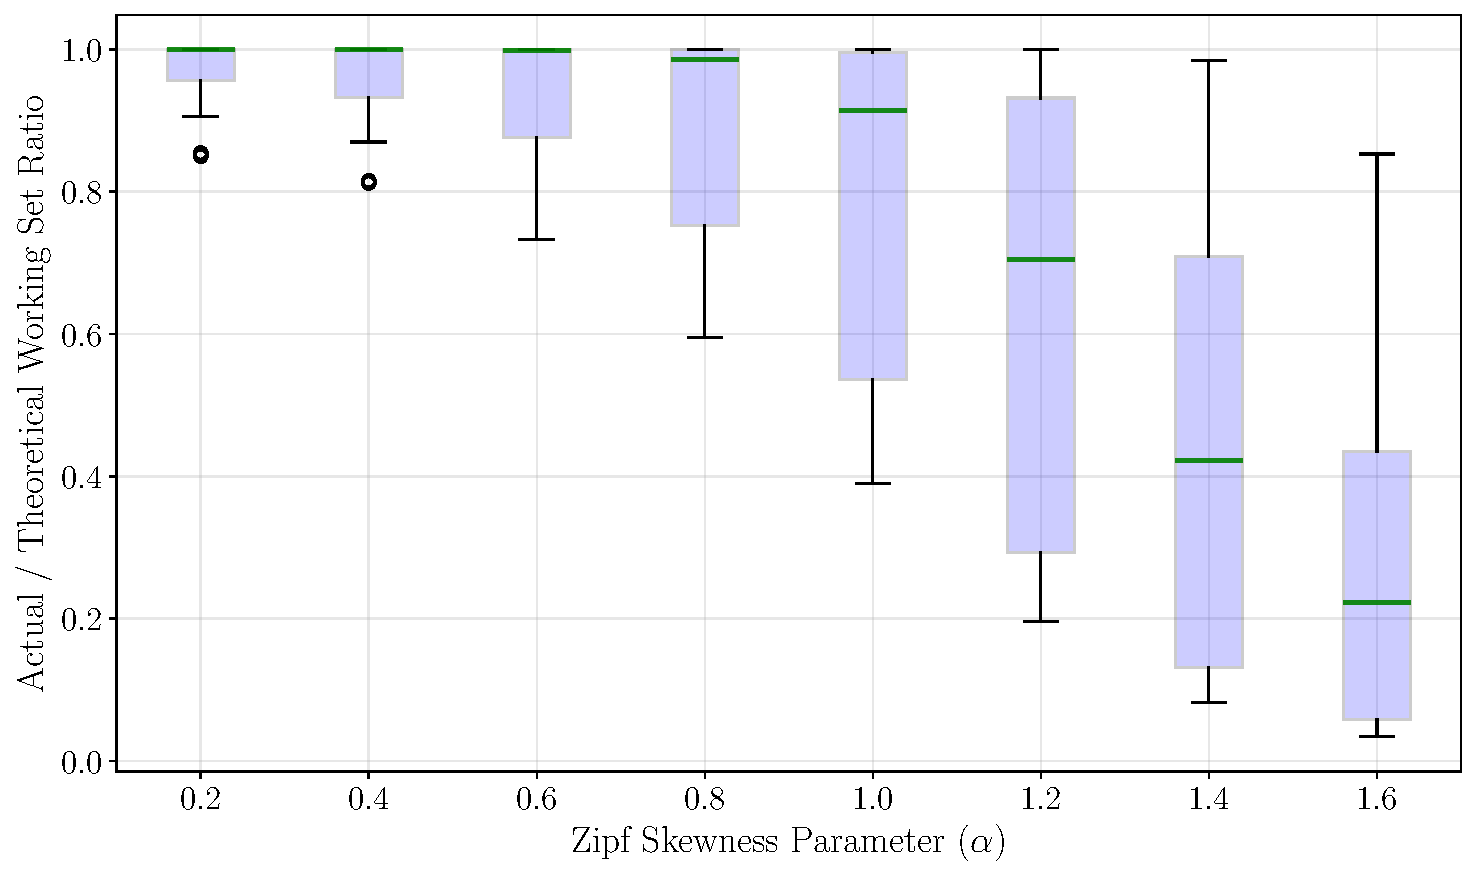
\includegraphics[width=0.8\linewidth]{figures/workloads/boxplot_alpha_vs_actual_theoretical_ratio.pdf}
    \label{fig:boxplot-actual-theoretical-ratio}
\end{figure}

From \Cref{fig:boxplot-actual-theoretical-ratio}, we observe that the skewness parameter $\alpha$ has a significant impact on the actual working set size generated. As $\alpha$ increases, the median ratio of the actual to the theoretical working set size decreases sharply. For a low skewness ($\alpha=0.2$), the median ratio is close to 1, indicating that most of the theoretical working set is captured. However, for a high skewness ($\alpha=1.6$), the median ratio drops below 25\%.

This phenomenon is due to the nature of sampling from a highly skewed distribution. A larger $\alpha$ means the distribution is more uneven, with a small number of items accounting for the majority of requests, while a long tail of very rare items exists. When a limited number of requests are sampled, it becomes increasingly difficult to encounter all of these rare items, leading to a smaller actual working set compared to the theoretical one.

Furthermore, we can see that a higher $\alpha$ value not only decreases the median ratio but also significantly increases the spread of the working set sizes, as evidenced by the widening interquartile range (IQR). For example, the less skewed distribution with $\alpha=0.2$ shows an IQR of around 1.5, while this IQR drastically increases to 8 for a more skewed distribution with $\alpha=1.6$. This wider spread suggests that for highly skewed distributions with large values for $\alpha$, the actual working set size can be highly variable depending on the specific sampling, highlighting the instability of the working set under these conditions.




%%%%%%%%%%%%%%%%%%%%%%%%%%%% CACHE SIMULATIONS

\section{Cache Simulations}\label{res:cache-sim}

This section outlines the experimental findings gathered from the cache simulations performed. We investigate findings regarding the miss ratio distribution of each algorithm before investigating the effects of the Zipfian skewness parameter $\alpha$ and the relative cache size on the measured miss ratios.

\subsection{Miss Ratio Distribution}\label{results:miss-ratio-distribution}

\outline{miss ratio distribution by algorithm}

As discussed in \Cref{subsec: cache-simulations}, a total of 28,851 cache simulations using unique configurations were performed on each algorithm. The miss ratio distribution for each algorithm (FIFO, LRU, SIEVE) is presented in the boxplot in \Cref{fig:miss-ratio-distribution}, with relevant miss ratio statistics outlined in \Cref{tab: miss_ratio_stats}.

\begin{figure}[h!]
    \centering
    \caption{Summary of Cache Algorithm Miss Ratio Statistics}
    \label{tab: miss_ratio_stats}
    \begin{tabular}{l r r r r r r r r}
        \toprule
        \textbf{Algorithm} & \textbf{Mean} & \textbf{Median} & \textbf{Std Dev} & \textbf{Min} & \textbf{Max} & \textbf{Q1} & \textbf{Q3} & \textbf{IQR} \\
        \midrule
        FIFO & 0.6386 & 0.7586 & 0.3384 & 0.0111 & 1.0000 & 0.3274 & 0.9671 & 0.6397 \\
        LRU & 0.6190 & 0.7318 & 0.3490 & 0.0089 & 1.0000 & 0.2780 & 0.9643 & 0.6863 \\
        SIEVE & 0.5779 & 0.6236 & 0.3491 & 0.0088 & 1.0000 & 0.2316 & 0.9274 & 0.6959 \\
        \bottomrule
    \end{tabular}
\end{figure}


\begin{figure}[h!]
    \centering
    \caption{Miss Ratio Distribution by Algorithm. The {\color{red}\textbf{red}} line represents the median.}
    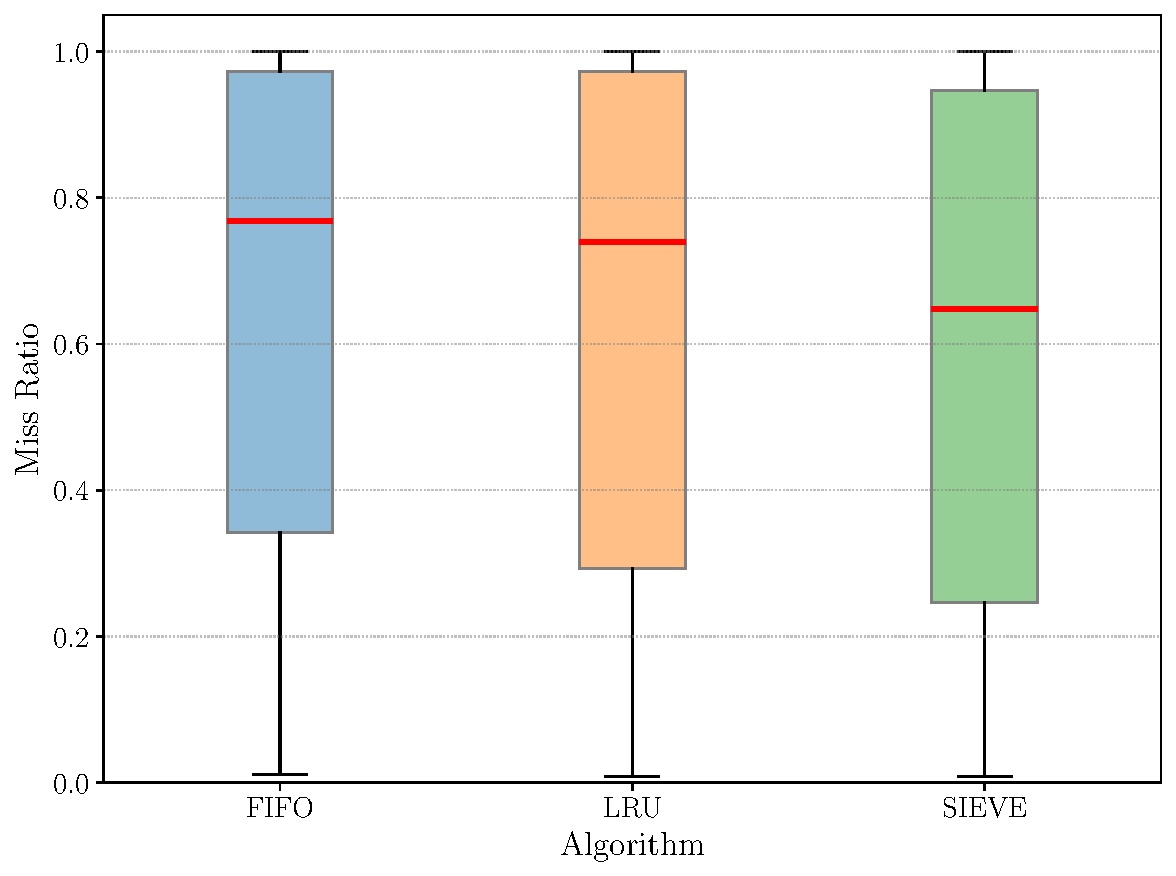
\includegraphics[width=0.6\linewidth]{figures/simulations/miss_ratio_distribution_no_title.pdf}
    \label{fig:miss-ratio-distribution}
\end{figure}

Based on the miss ratio boxplot (\Cref{fig:miss-ratio-distribution}) and accompanying table (\Cref{tab: miss_ratio_stats}) with relevant statistics, there is a clear performance hierarchy among the algorithms, with SIEVE generally outperforming the others. The median miss ratios show this trend: with a median miss ratio of around 0.62, SIEVE demonstrates a measurable advantage to its competitors, with LRU's median miss ratio being approximately 17\% higher and FIFO about 22\% higher than SIEVE's. This confirms that SIEVE, on average, handles all Zipf-like workloads, regardless of parameters, more efficiently than LRU and FIFO.

The mean miss ratios support this finding. SIEVE has a mean of around 0.58, which is lower than LRU (0.62) and FIFO (0.64). This suggests that SIEVE's performance is consistently better across the full range of simulations, followed by LRU.

All three algorithms exhibit a wide range of performance. The standard deviations are all relatively high (around 0.34), and the interquartile ranges (IQR) are broad, suggesting that the miss ratio for any given algorithm can vary significantly depending on the specific workload configuration. For example, all three algorithms have a minimum miss ratio close to zero and a maximum of 1.0, suggesting their sensitivity to other factors. Nevertheless, it is interesting to observe that SIEVE demonstrates the highest variability compared to the baselines, with slight differences in its standard deviation: approximately 3.07\% greater than FIFO and 0.04\% greater than LRU.

Though all algorithms show a similar high degree of variability, SIEVE demonstrates a measurable advantage in terms of both median and mean miss ratio performance, indicating its strength when applied to Zipf-like distributions. Nevertheless, it is interesting to further investigate the cause for this high variability of miss ratios among all algorithms.

\subsection{Effect of Zipfian Skewness Parameter ($\alpha$) on Miss Ratio}\label{results:alpha-miss-ratio}

\outline{miss ratio vs. alpha}

The large variability in miss ratios can be directly linked to changes in the Zipfian skewness parameter ($\alpha$) used during workload generation. \Cref{fig:miss-ratio-vs-alpha} demonstrates the effect of $\alpha$ on the miss ratio. The exact values obtained for the mean miss ratio can be found in \Cref{appendix:miss-ratio-alpha}.

\begin{figure}[h!]
    \centering
    \caption{Miss Ratio vs. Zipf Skewness Parameter $\alpha$}
    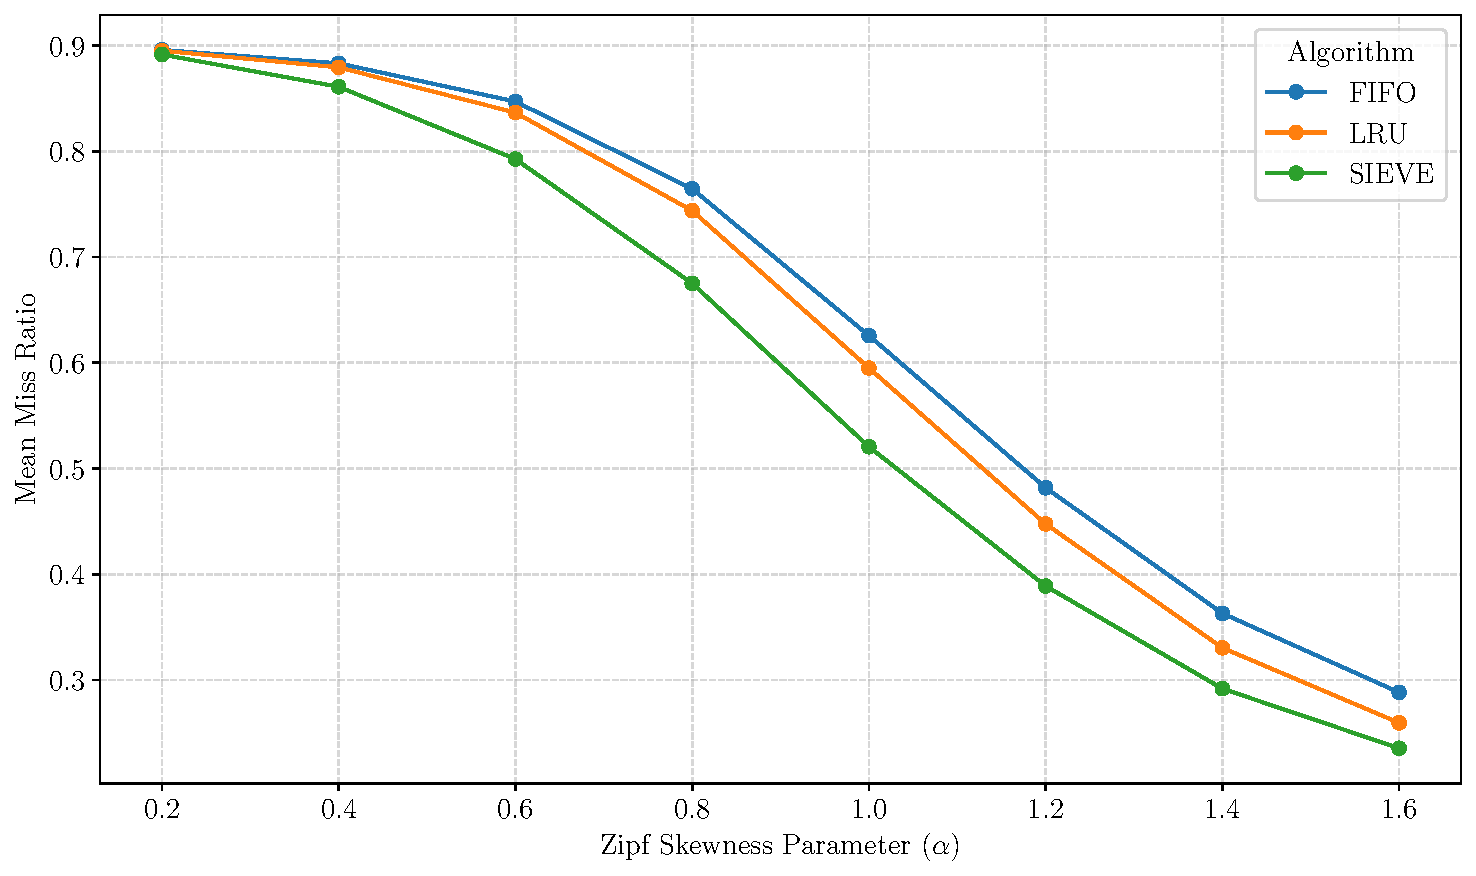
\includegraphics[width=0.8\linewidth]{figures/simulations/miss_ratio_vs_alpha_no_title.pdf}
    \label{fig:miss-ratio-vs-alpha}
\end{figure}

From \Cref{fig:miss-ratio-vs-alpha}, we can observe that, regardless of the algorithm used, the graph follows a downward-sloping curve. This demonstrates a crucial relationship: as $\alpha$ increases, the miss ratio decreases. This is a direct consequence of the nature of a Zipfian distribution: higher $\alpha$ values result in a more skewed distribution, where a small number of items are requested far more frequently. This concentration of requests on a few popular items leads to a greater number of cache hits and, consequently, a lower overall miss ratio.

When considering the performance of the different algorithms in \Cref{fig:miss-ratio-vs-alpha}, SIEVE consistently outperforms LRU and FIFO across all tested $\alpha$ values. This finding aligns with the general miss ratio distribution results discussed in \Cref{results:miss-ratio-distribution}, where SIEVE exhibited the lowest median miss ratio in general. The performance gap between SIEVE and the other algorithms is most pronounced in the mid-range of $\alpha$ values, particularly from $\alpha=0.8$ to $\alpha=1.2$. SIEVE's performance advantage is more visually apparent in \Cref{fig:sieve-advantage}, which plots the percentage advantage in miss ratio that SIEVE holds over FIFO and LRU.

\begin{figure}[h!]
    \centering
    \caption{Miss Ratio Performance Advantage of SIEVE Algorithm}
    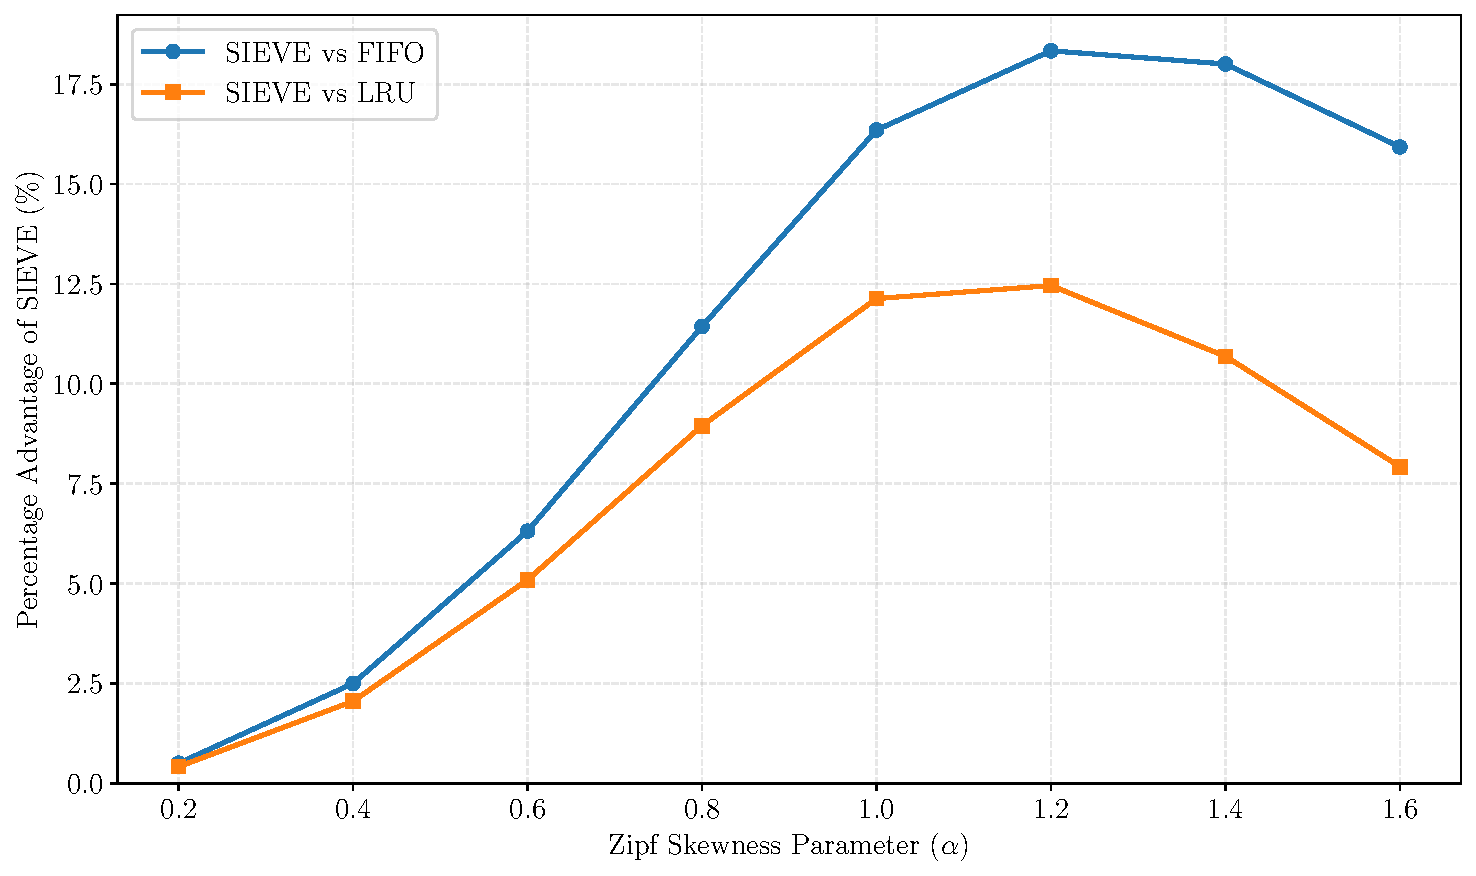
\includegraphics[width=0.8\linewidth]{figures/simulations/sieve_advantage_no_title.pdf}
    \label{fig:sieve-advantage}
\end{figure}

\Cref{fig:sieve-advantage} shows that SIEVE's outperformance is not uniform. The miss ratio advantage peaks in the mid-range of $\alpha$ values. Specifically, the maximum advantage over LRU is approximately 14\% at $\alpha=1.2$, while the maximum advantage over FIFO is slightly above 20\% at the same $\alpha$ value. This suggests that SIEVE is particularly effective at managing highly skewed workloads, where a balance is needed between caching the few very popular items and the large number of less popular items. At low levels of skewness (at $\alpha=0.2$), the performance advantage of SIEVE is less prevalent, but as skewness increases, so does the performance difference between the algorithms.


\subsection{Effect of Relative Cache Size on Miss Ratio}\label{results:miss-ratio-vs-relative-cache-size}

\outline{miss ratio vs. relative cache size}

Aside from the Zipfian skewness parameter $\alpha$ having a notable effect on the miss ratio of all algorithms, the relative cache size also has a significant impact. \Cref{fig:miss-ratio-cache-size} demonstrates a meaningful relationship between the relative cache sizes and the resulting mean miss ratio measured. The specific values measured can be found in \Cref{appendix:rel-cache-size}.

\begin{figure}[h!]
    \centering
    \caption{Miss Ratio vs. Relative Cache Size}
    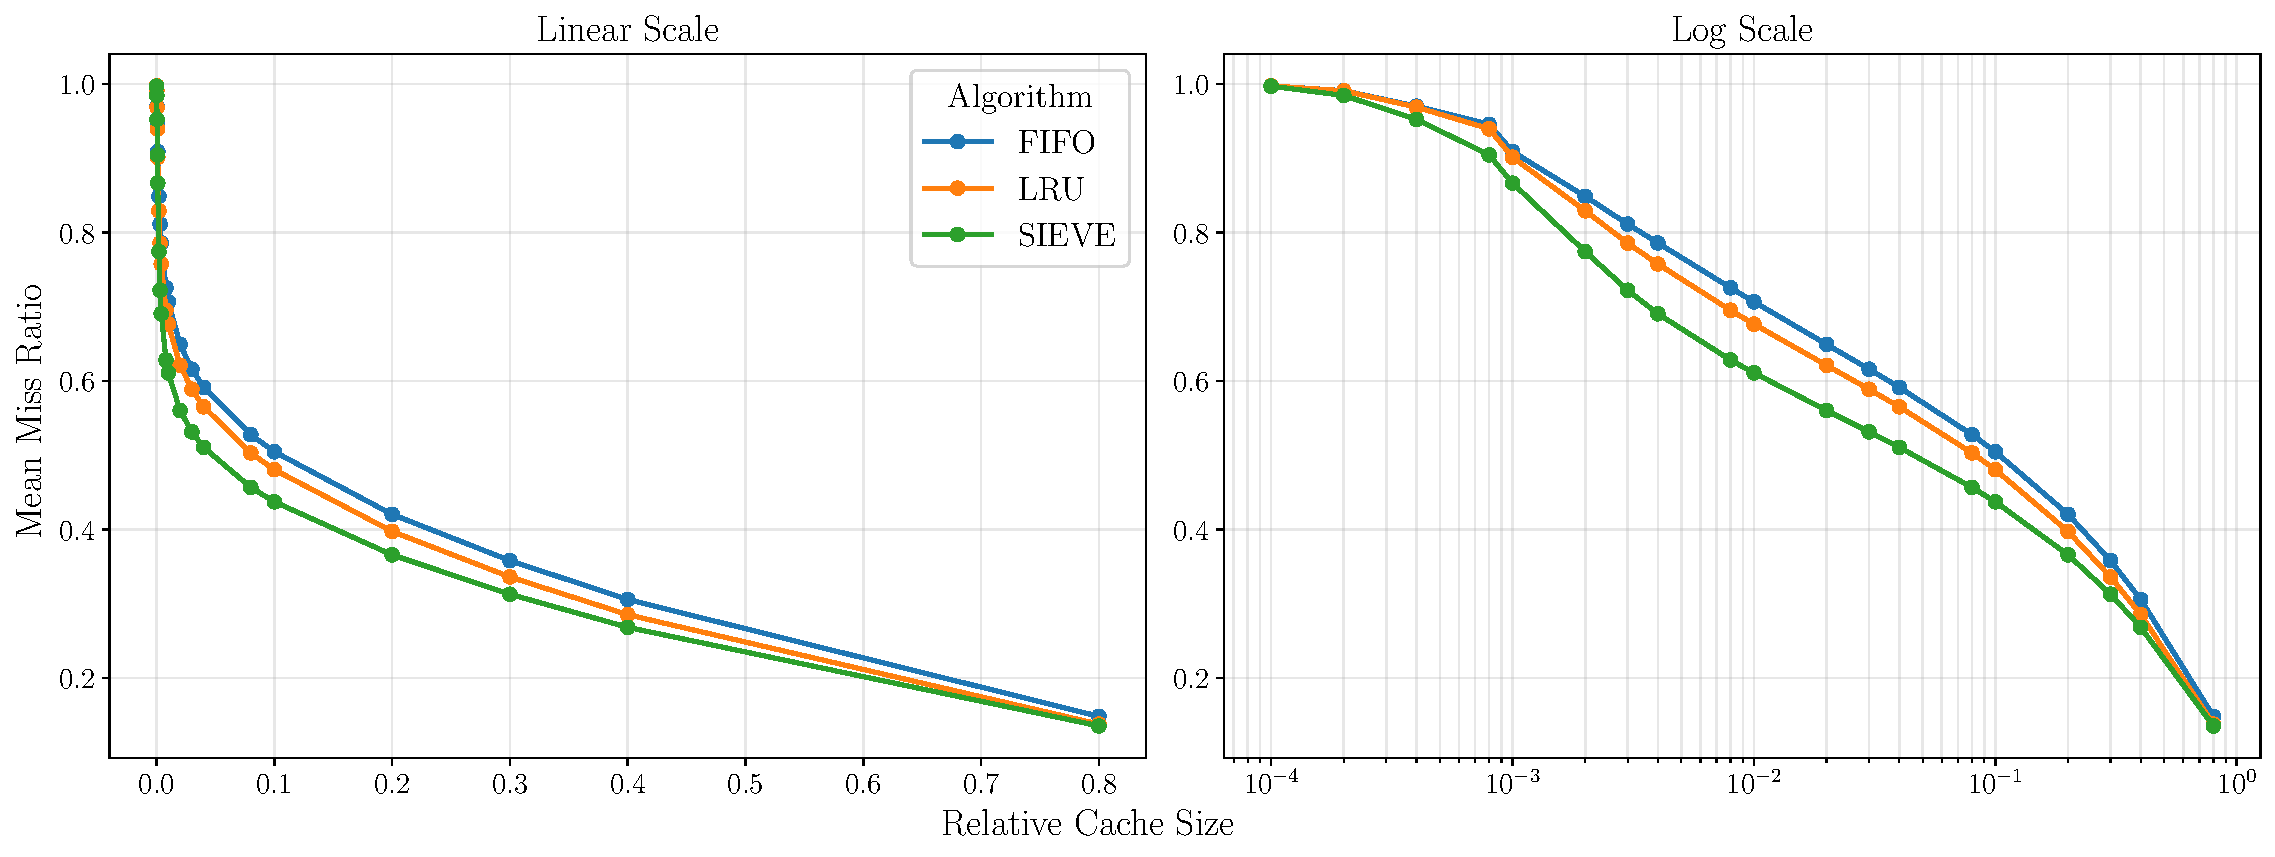
\includegraphics[width=\linewidth]{figures/simulations/miss_ratio_vs_cache_size_both.pdf}
    \label{fig:miss-ratio-cache-size}
\end{figure}

As shown in the linear scale plot in \Cref{fig:miss-ratio-cache-size}, the mean miss ratio consistently decreases with increasing relative cache size. However, the rate of this decrease is highly non-linear. The initial sharp drop in the miss ratio for relative cache sizes of 0.0001 to 0.02 (highlighted range) indicates that small increases in cache size yield significant performance improvements, with a decrease in the mean miss ratio of 0.23 from around 1.00 to 0.77 for SIEVE.

Beyond a relative cache size of 0.1, the rate of improvement diminishes considerably. For example, a larger increase of the relative cache size from 0.1 to 0.2 results in a much smaller reduction in miss ratio of 0.07, dropping from about 0.44 to 0.37 for SIEVE. This suggests a point of "diminishing returns" where further increases in cache size offer only marginal performance gains. The log scale plot on the right further highlights this non-linear relationship more clearly, visually stretching out the initial region of rapid performance gain and compressing the later region where gains are minimal.

Furthermore, when considering the relative performance of the three cache primitives, we see that SIEVE consistently maintains the lowest mean miss ratio across all relative cache sizes. For example, at a relative cache size of 0.2, SIEVE's miss ratio advantage is most notable: around 10\% better than LRU's and 14\% better than FIFO's.

\subsection{Relationship Between $\alpha$ and Relative Cache Size}

\outline{miss ratio heat map}

The results demonstrated above, in \Cref{results:alpha-miss-ratio} and \Cref{results:miss-ratio-vs-relative-cache-size}, both reveal that independent of $\alpha$ and the relative cache size, SIEVE consistently outperforms LRU and FIFO. Rather than focusing on differences between the algorithms, the heatmap from \Cref{fig:miss-ratio-heatmap} underlines the meaningful relationship between $\alpha$ and the relative cache size on the resulting mean miss ratio of all algorithms. Each data point on the plot represents the mean miss ratio for a specific combination of $\alpha$, relative cache size, and caching algorithm (FIFO, LRU, and SIEVE). The shape of the point (round, square, triangle) determines the algorithm used, and the color determines the relative cache size (lighter colors indicate a larger size).

\begin{figure}[h!]
    \centering
    \caption{Mean Miss Ratio vs. Zipf Skewness Parameter ($\alpha$) and Relative Cache Size}
    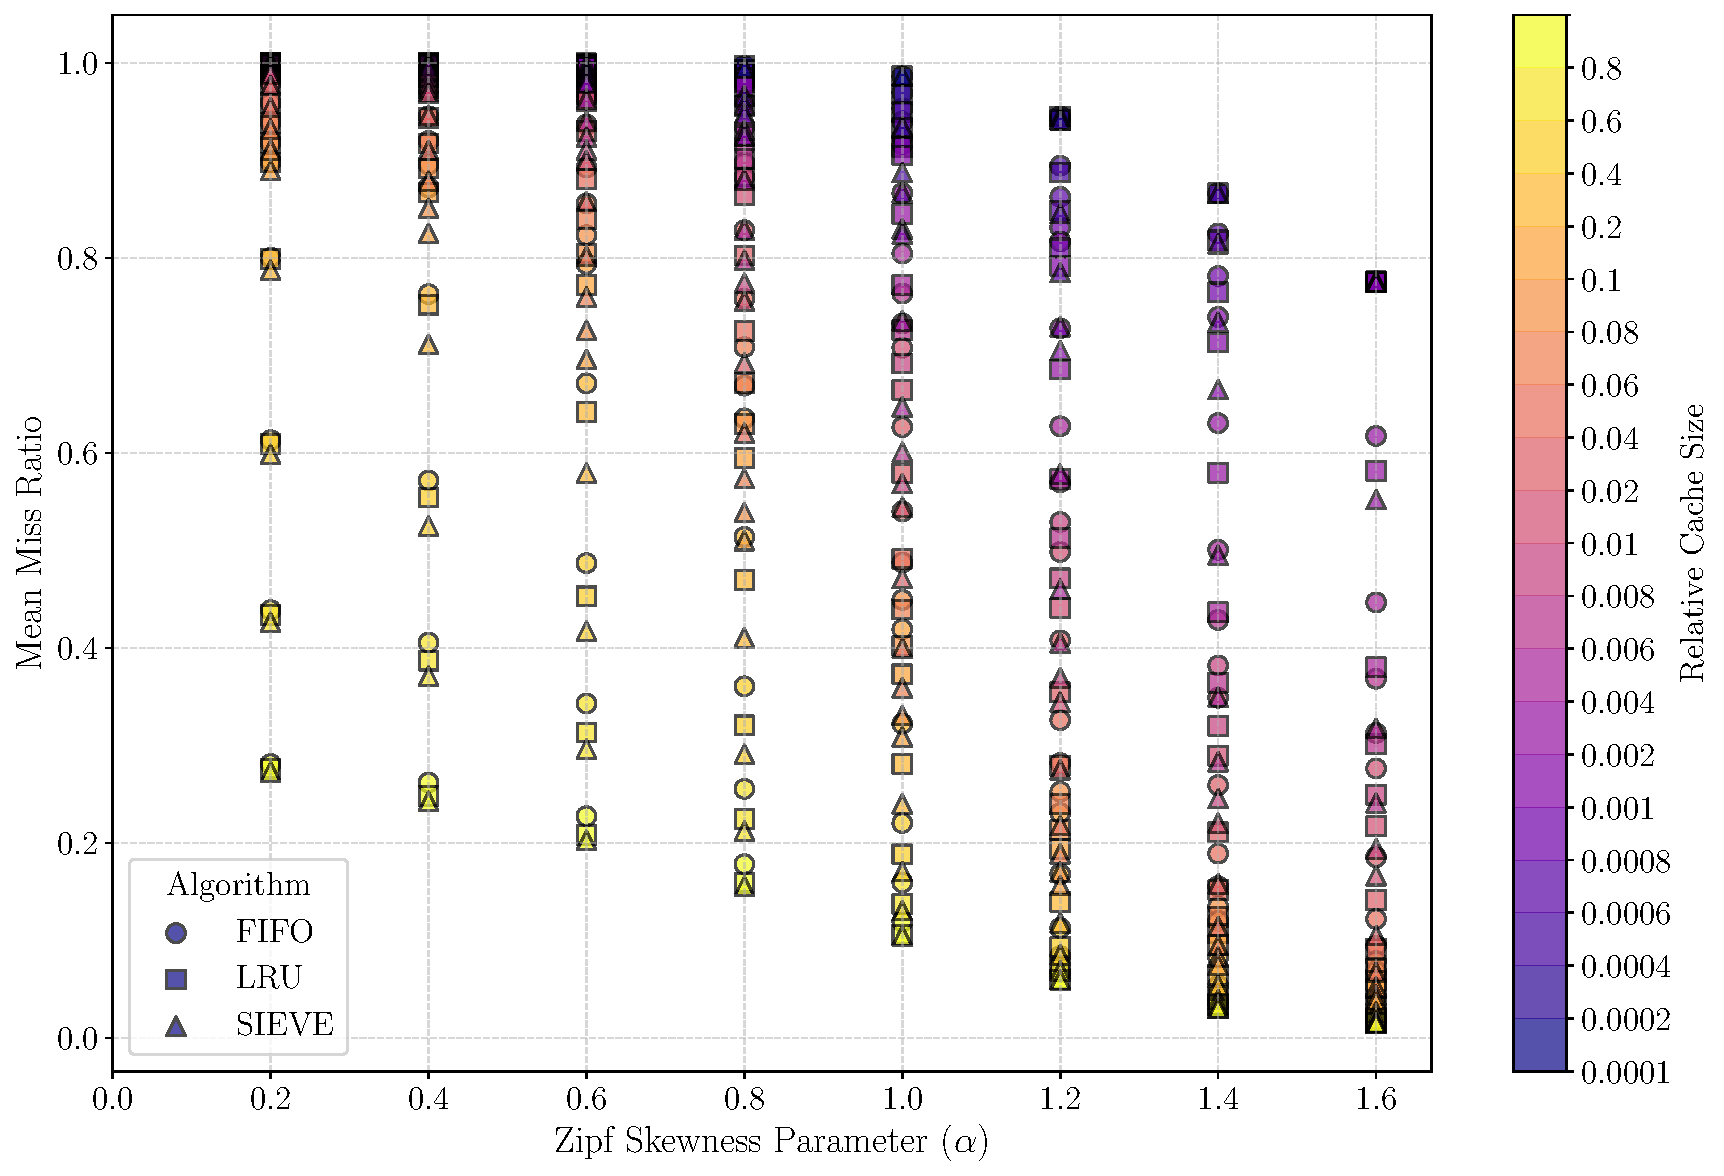
\includegraphics[width=\linewidth]{figures/simulations/miss_ratio_heat_map_no_title.pdf}
    \label{fig:miss-ratio-heatmap}
\end{figure}

A clear visual pattern emerges from the data demonstrated in \Cref{fig:miss-ratio-heatmap}: an inverse relationship between the miss ratio to $\alpha$ and the relative cache size. Regardless of algorithm, the optimal performance is achieved at high values for $\alpha$ and relative cache size.

The larger cache sizes (yellow and light orange points) consistently result in a lower miss ratio across all $\alpha$ values. The most significant reduction in miss ratio occurs as the cache size increases, particularly in the mid-range of $\alpha$ values ($\alpha=0.8$ to 1.2), where the workload is skewed enough to be captured by a reasonably sized cache, but not so extreme that a tiny cache is sufficient. The large vertical spread of points at each $\alpha$ value reinforces the strong influence of cache size on the efficiency of any cache eviction algorithm.

We further observe that as $\alpha$ increases, the distribution of mean miss ratios by relative cache size also changes. For lower $\alpha$ values, smaller cache sizes perform notably worse than at higher $\alpha$ values. For example, at $\alpha = 0.2$, relative cache sizes less than around 0.1 do not surpass a miss ratio of 0.8. However,  at $\alpha = 1.6$, every relative cache size accounted for achieves a miss ratio of less than 0.8. Here, we learn that a more skewed workload allows smaller cache sizes to perform better.
